\chapter{xHCI Stack Implementation}

The structure of the xHCI driver is quite straightforward, as it tries to fit
into the scheme of how hardware and the rest of HelenOS works. We decided to
use the existing library \lib{libusbhost} to reduce code duplication with
other HC drivers. IT came out that this library need a lot of changes to
support us in this goal, but that's for chapter \ref{usb-refactoring}.

The USB host controller driver using \lib{libusbhost}, xHCI included, serves as
a connecting layer between the hardware and library, and exposes its bus
interface.

\begin{figure}[h]
	\centering
	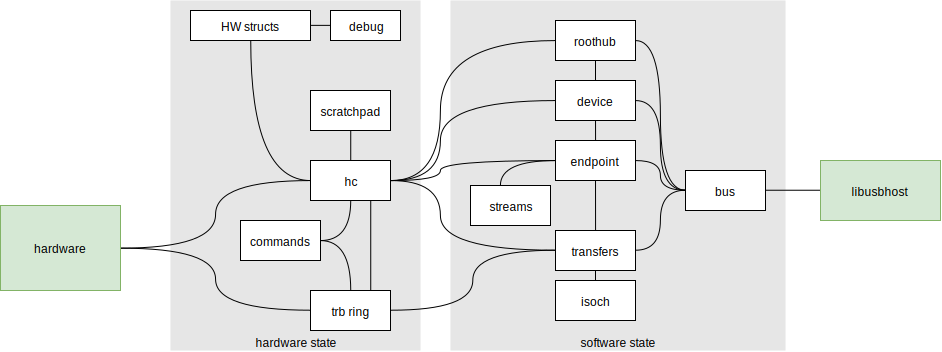
\includegraphics[width=0.8\textwidth]{xhci-architecture}
	\caption{The modules of xHCI driver}
\end{figure}

The scheme is not at all strict, we're in a C world, there are dependencies
almost everywhere -- take it as an informal overview to get an idea.

The whole driver can be split into two parts. The left one takes care about the
hardware perception on what's going on, the right one is about managing the
software structures and memory.

We start with describing the modules in the hardware part, as their
functionality is clear. Their order follows the order in which they were
implemented.

\section{HW structs}

% TODO: Explain that this one is really simple, and just mirrors the structures
% hardware use.

\section{Debug}

% TODO: Describe that we used it during debugging to check what we're doing.

\section{TRB ring}

% TODO @aearsis: explain the TRB rings, what they do and how they're
% implemented (ْ±2 pages, bore the reader to death right now!)
\subsection{Purpose}
\subsection{Implementation}

\section{Scratchpad}

% TODO: Anyone please explain these. The only interesting part is how the
% number of buffers are split weird and how we needed several attempts to get
% it right :)

\section{Events}

% TODO: Explain events, event handling and the event ring.


\section{Commands}

The xHC offers an independent command interface. During operation, the xHC
driver uses this interface to manipulate device slots, devices and endpoints by
executing various commands provided by a unified the command subsystem. This
section provides details on the structure and implementation of this subsystem.


\subsection{Execution Workflow}

The xHC command interface consists of a TRB command ring and a command doorbell
register. Commands are executed by placing various command TRBs onto this ring,
forming a \textit{Command Descriptor}.

After placing the respective TRBs and writing into the xHC command doorbell
register, the descriptors on the command ring are sequentially processed by the
xHC, resulting in either failure or successful completion. The result of every
command descriptor is reported back to the xHC driver in the form of a
\textit{Command Completion Event} placed onto the primary event TRB ring.

After writing into the xHC command doorbell register and before receiving the
respective command completion event, the xHC driver can attempt to abort the
issued command. Such action might be of use for instance if the command
completion event does not arrive within a set time period.

Note that this section intentionally omits hardware technical details, which are
not instrumental to understanding the command subsystem. For further hardware
documentation of the xHC command interface, refer to Section 4.6 of the xHCI
specification.


\subsection{Structure}

The xHC driver command subsystem instance is represented by the
\struct{xhci_cmd_ring_t} structure which exists throughout the entire duration
of the xHC driver's lifecycle. The purpose of this structure is to maintain and
manage the command TRB ring, and to keep track of enqueued command descriptors.

Individual command descriptors are represented by the \struct{xhci_cmd_t}
structure. In it are stored the high-level parameters of the command as well as
the command TRB, which is placed onto the command ring when the command is
executed. While the high-level command parameters are kept directly in this
structure, the hardware-related internals are kept in a substructure, which is
commonly referred to as \textit{command header}. The purpose of this separation
is to stress that the header contents are to be exclusively accessible to the
command subsystem only, while the rest of the structure remains accessible to
the entire xHC driver.

Besides data structures, the command subsystem offers a centralized command
completion event handler function -- \fnc{xhci_handle_command_completion()} --
which is called by the event subsystem in case a \textit{Command Completion
Event} is encountered.

The last major component of the command subsystem are functions used to generate
and schedule commands on the xHC. These functions produce valid instances of the
\struct{xhci_cmd_t} and place their respective TRBs onto the command ring
managed by the \struct{xhci_cmd_ring_t} structure, requesting either blocking or
non-blocking semantics for waiting on their completion. These functions are
described detail in the next section.


\subsection{Implementation}


% TODO @dzejrou or @petr: Explain why commands are needed and the basic
% structure of the subsystem

% TODO @petr: Show off with the inline syntax

\subsubsection{Aborting commands}

% TODO @aearsis: Explain the arcane magic behind aborting commands.

\section{Host controller module}

% TODO: This will be harder, this one is a mix of what didn't fit anywhere else.
% Ideas:
% - event handling
% - context management
% - extcap parsing
% - register access macros

\section{Roothub}

% TODO: Explain why we do not have virthub. Who remembers the reasons?
% Otherwise it just uses libusb/port to do the interesting work.

\section{Transfers}

% TODO @salmelu (probably?): Write something about it.

\subsection{Isochronous transfers}

% TODO @salmelu: Copy that from the wiki :)

\section{Bus module}

% TODO: After the device will be split, will there be anything interesting to write about?

\subsection{Device}

% TODO: Enumeration, device context

\subsection{Endpoint}

% TODO: Contexts, rings

\subsection{Streams}

% TODO @salmelu: Noone else understands that now.
